\newpage

\section{Conclusion and future plans}

While designing and working on this project we learned a lot about the inner workings of
car ECUs, communication and PCB design. This project provided unique challenges, of which
the biggest one was tackling the lesser known and documented (in French no less) VAN protocol.
We have already started working on the next revision of the board as well as the next step in
this project. Since we are piggybacking on the existing display in the car, the next step
is reverse engineering the logic of the display and completely replacing it. That, however, is
for another time.

\bigskip
\noindent
Another challenge that had to be tackled for this project, but wasn't mentioned as much, was
building a custom Linux distribution for the Raspberry Pi. That will be expanded upon
in the next iteration of this project.

\begin{figure}[H]
    \begin{center}
        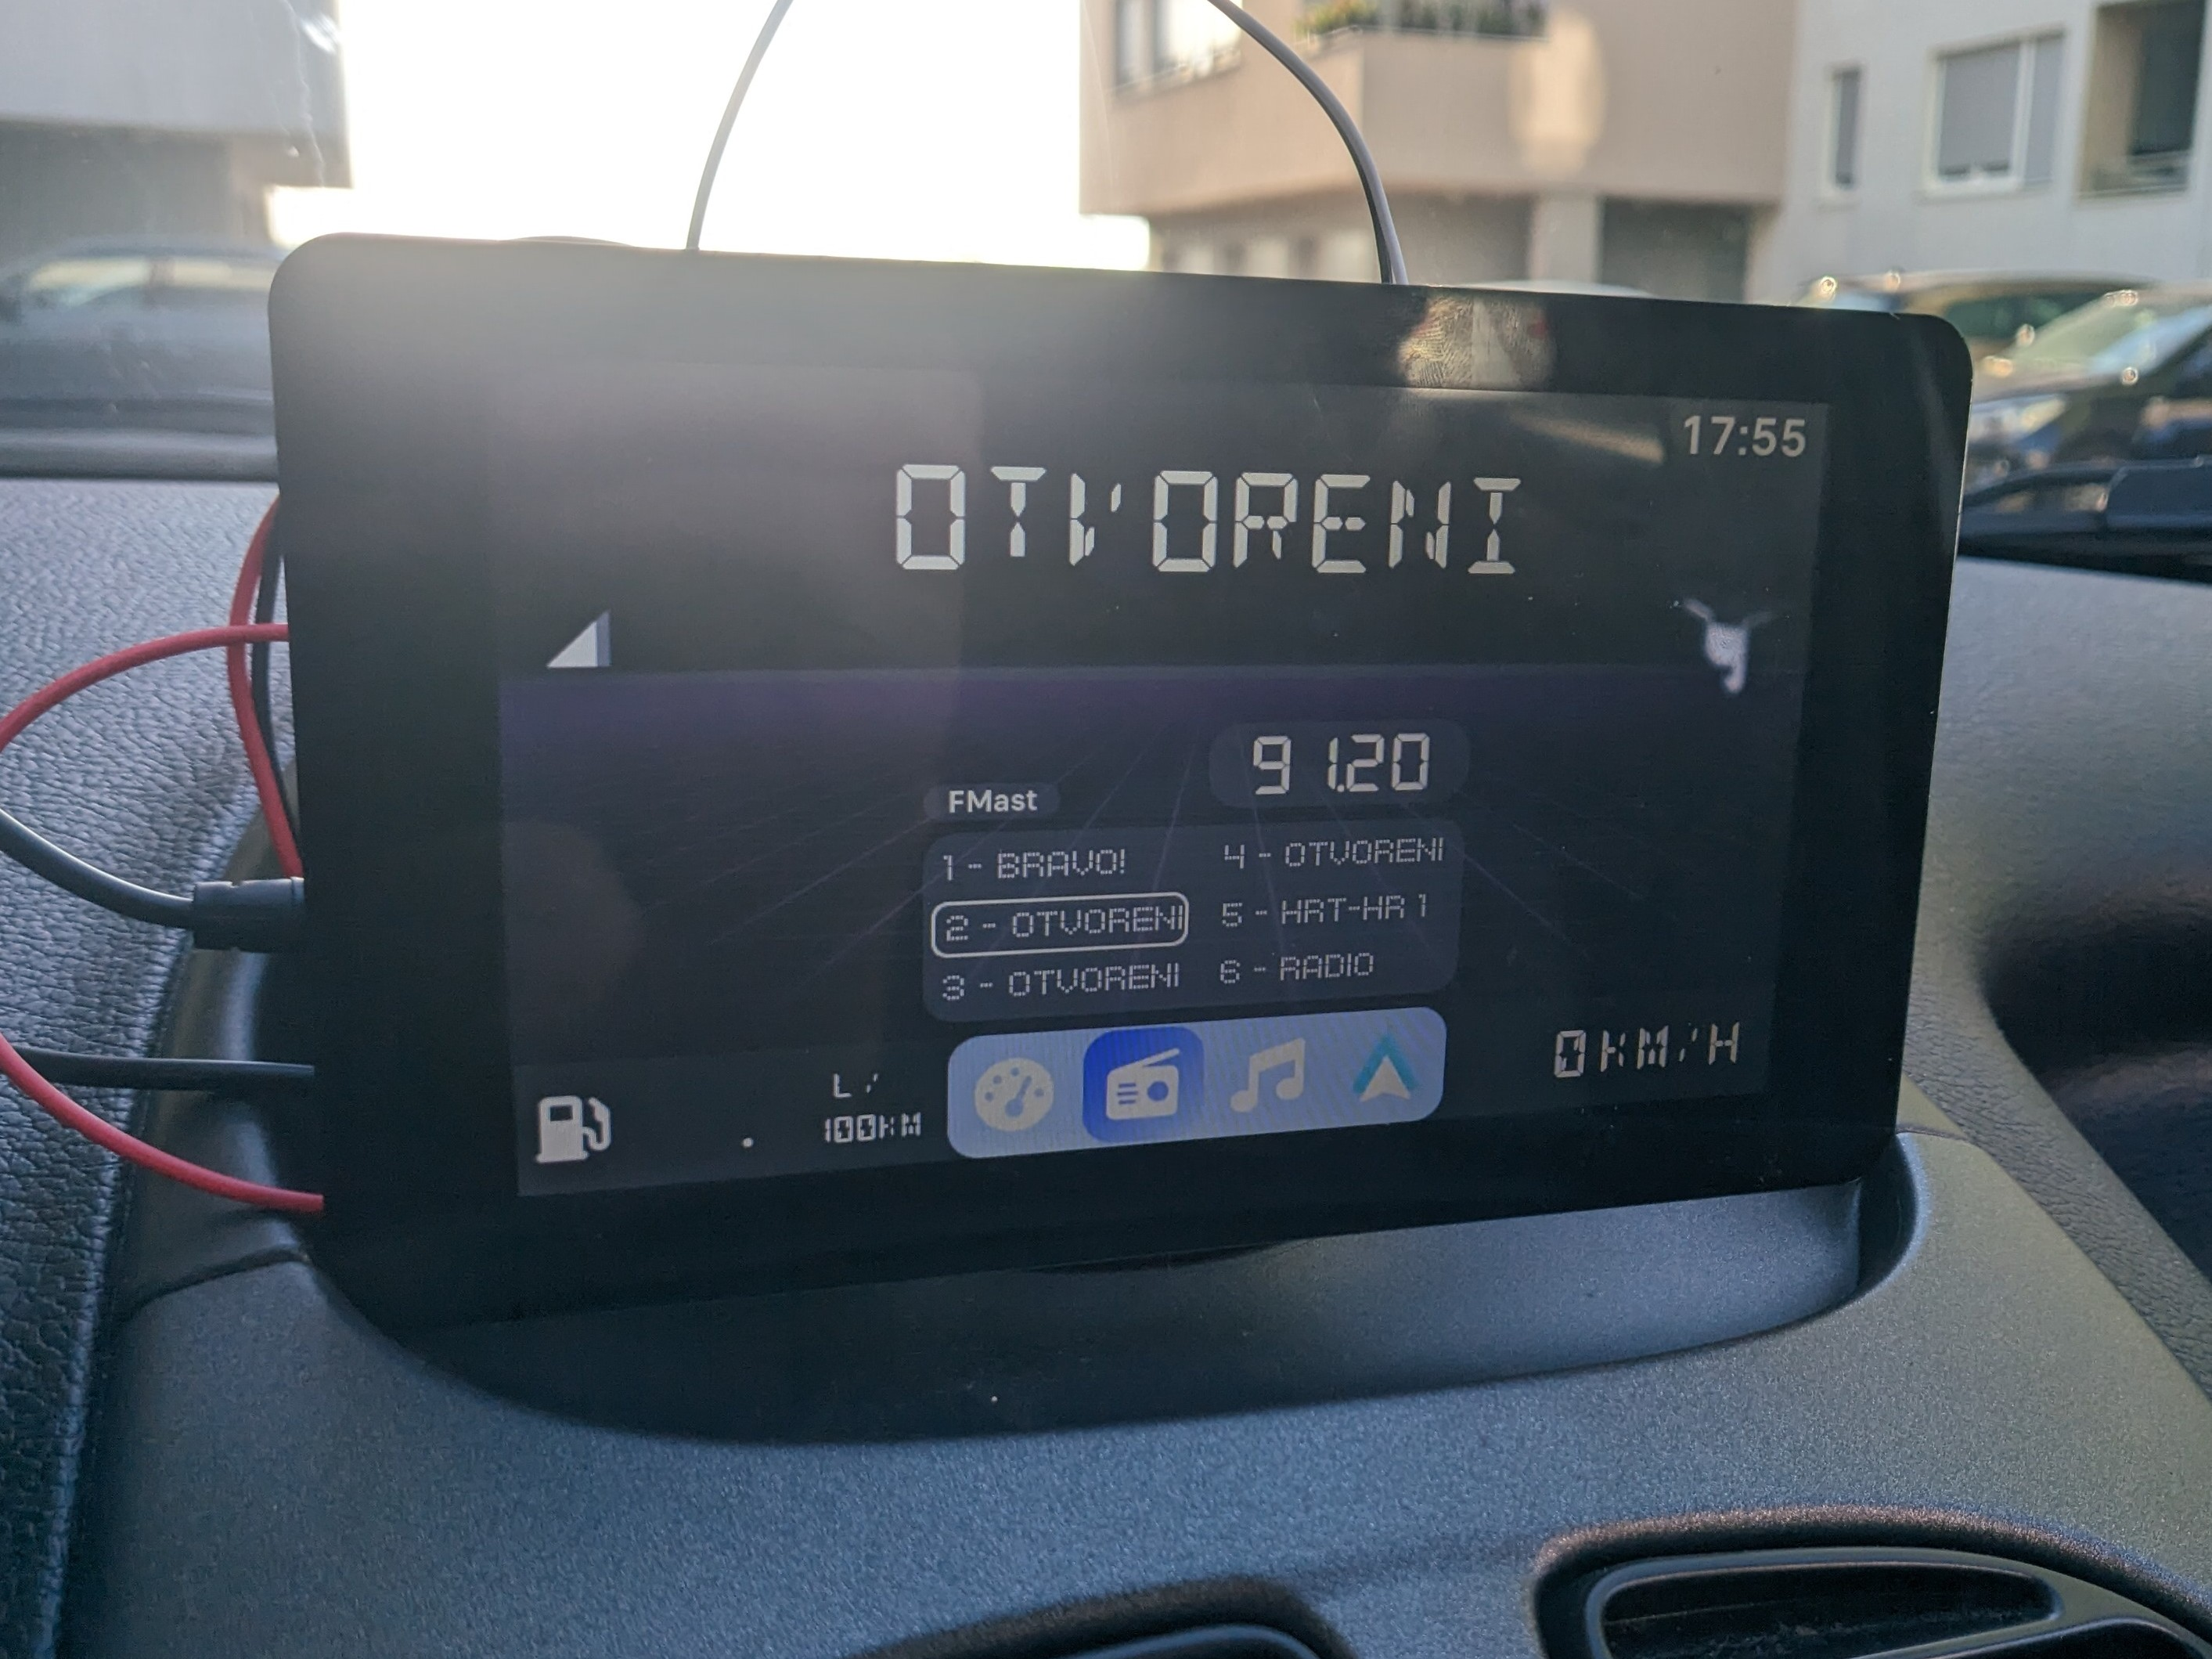
\includegraphics[width=0.75\textwidth]{images/PXL_20250825_175514473.jpg}
        \caption{Infotainment system placed in the car}
    \end{center}
\end{figure}